\documentclass[conference]{IEEEtran}
\usepackage{blindtext, graphicx}
\usepackage{cite} 
\usepackage{csquotes}
\usepackage[hidelinks]{hyperref}
\usepackage{url}

\hyphenation{op-tical net-works semi-conduc-tor}

\begin{document}
\title{A Comparative Analysis of Vision-Based and GPS-Based Speed Estimation Algorithms for Autonomous Vehicles}

% The sequence of authors in a paper has meaning. The first to be listed is known as the First Author, who is usually the student and/or the person doing the bulk of the work. The next in line, provided that there are two persons, is called the corresponding author, also known as the technical mentor/supervisor. Any person who is consulting, correcting or verifying such as a second reader or senior person within the Faculty/Institute is listed after the previous authors.

\author{\IEEEauthorblockN{Denzel Baldacchino}
\IEEEauthorblockA{Institute of Information \& Communication Technology\\
Malta College or Arts, Science \& Technology\\
Corradino Hill\\
Paola PLA 9032\\
denzel.baldacchino.g52078@mcast.edu.mt}}

\maketitle

% \begin{abstract}
Accurate estimation of vehicle speed is fundamental to autonomous navigation. This study critically evaluates the precision of a vision-based Dense Optical Flow (Farnebäck) algorithm, augmented with dynamic affine calibration, in comparison to consumer-grade GPS trajectory data. Utilizing the comma2k19 dataset, both methodologies were assessed against a 100Hz CAN-bus ground truth within a dynamic urban driving environment. A quantitative approach was employed, involving the calculation of Mean Absolute Error (MAE), Root Mean Square Error (RMSE), and Mean Bias Error (MBE). The findings definitively refuted the initial hypothesis: the GPS-based approach considerably outperformed the vision system, recording an MAE of 1.68 km/h in contrast to 4.50 km/h. Whilst GPS demonstrated considerable robustness across varying environmental conditions, the pure pixel-tracking vision method proved exceptionally vulnerable to visual noise, such as shadows, and failed to reliably detect deceleration. The study concludes that standard GPS probe data is markedly superior to Dense Optical Flow for vehicle speed estimation. Future research should focus on Sensor Fusion techniques, integrating deep learning models (such as YOLO) and Kalman filtering, to address the inherent limitations of both technologies.
\end{abstract}

\IEEEpeerreviewmaketitle

\section{Introduction}
\label{sec:Int}
\subsection{Theme \& Topic Rationale}
\par This research focuses on the theme of Intelligent Transport Systems (ITS) and Autonomous Vehicle Sensor Perception. Getting an accurate estimate of a vehicle’s speed is super important for safety, especially for Advanced Driver Assistance Systems (ADAS) and autonomous navigation. While GPS is widely used, they frequently encounter signal degradation in urban canyons, tunnels, or adverse weather conditions, which can cause errors due to signal reflections (multipath errors) \cite{cui2003autonomous,li2025statistical}. On the other hand, estimating speed using dashcam footage is a cheaper, sensor-rich option \cite{pp2024video}, but it is inherently vulnerable to variations in lighting and computational latency. It’s important to compare these two methods against a highly accurate baseline, specifically vehicle CAN-bus data. Such comparison elucidates the specific environmental limitations of each system and offers empirical evidence to inform the development of improved algorithms in the future.
\subsection{Positioning \& Research Onion}
\par Based on Saunders’ Research Onion \cite{saunders2019research}, this research uses positivism, meaning seeing reality as something objective and separate from what other people think or interpret. The data that will be used is mainly measurable data like speeds, GPS coordinates and pixel shifts, with the researcher acting as an impartial observer by analysing the physical data. This research takes a deductive approach starting with already proved formulae and concepts such as the Haversine formula for GPS speeds and ego-motion tracking and comparing the data with each other to see which is more accurate. Even though the data comes from an archived source (Comma2k19) \cite{schafer2018commute}, the main objective for this research is to compare two algorithms under controlled conditions, using a steady CAN-bus ground truth to see how much error each algorithm has. Methodologically, the data is all quantitative because we are turning visual and geospatial information into numbers to analyse and compare statistically meaning there isn’t any qualitative data involved. The analysis is cross-sectional, so we are looking at a specific snapshot of data to test how well the algorithms work now, rather than tracking changes over time. Finally, we are collecting secondary data like video clips and GNSS logs to analyse and find the Mean Absolute Error for both algorithms.
\begin{figure}[htbp]
    \centering
    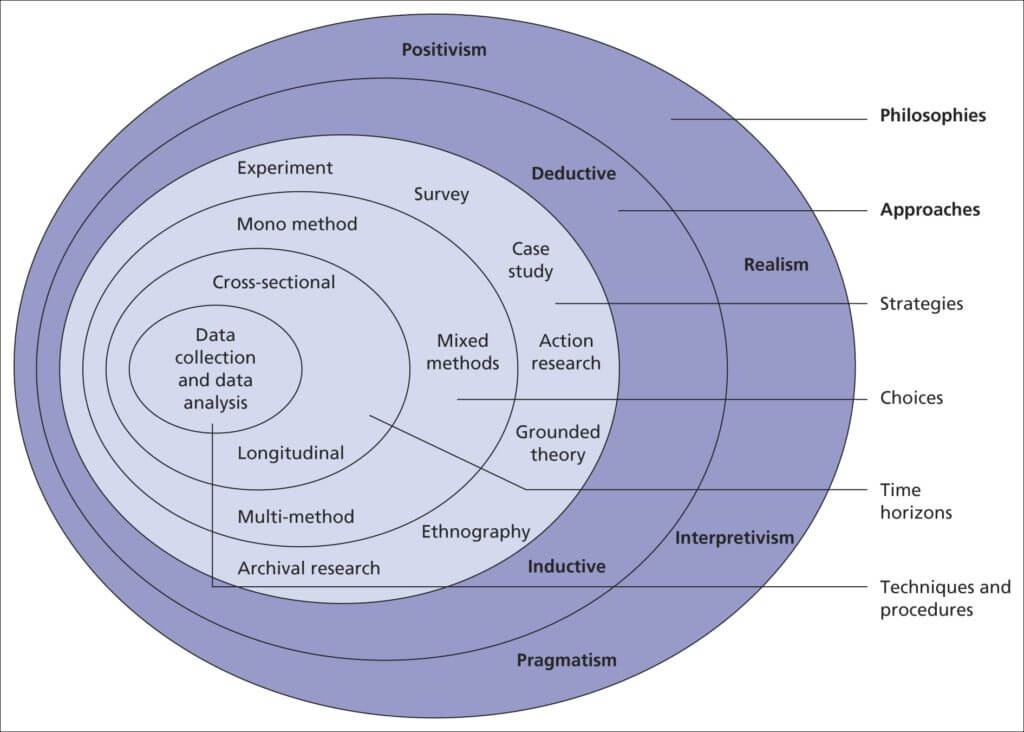
\includegraphics[scale=0.25]{includes/researchonion.jpg}
    \caption{Research Onion \cite{saunders2019research}}
    \label{fig:Onion}
\end{figure} 
\subsection{Background To This Research Theme}
\par The push towards fully autonomous vehicles has sped up the need for robust environmental awareness. In the past, navigation and speed checks have mostly relied on standard GPS receivers. But since self-driving technology needs accuracy to be down to milliseconds, the usual GPS signals and their delays or noise are not good enough \cite{cui2003autonomous}. Currently, recent advances in computer vision have made it possible to figure out “ego-motion”, basically how a camera moves through 3D space by tracking features \cite{pp2024video}. GPS can fail under bridges and cameras don’t work well in the dark or when there is lots of glare due to these drawbacks relying on just one sensor isn’t ideal thus the industry is leaning more towards combining different sensors. To manage to incorporate that well, researchers need to first understand how accurate each sensor is on its own and what kind of errors they might have when tested on real-world situations.
\subsection{Hypothesis}
\par This research works with a clear null hypothesis, which basically says there is no real difference in how accurate the vision-based algorithm is compared to GPS when it comes to estimating the vehicle’s true ground speed. On the other hand, the alternative hypothesis suggests that the vision-based method will have a smaller error margin than GPS during normal driving, mainly because commercial GPS units tend to have some delay and noise in their readings.
\subsection{Research Aim \& Purpose Statement}
\par The main goal of this study is to compare how accurately a vision-based speed estimation algorithm works versus a GPS-based one, using real-world dashcam footage. Ultimately, we are trying to spot the differences in how both methods measure speed. By testing against a solid ground truth, we hope to get useful insights into how reliable these sensors are, which could help in building safer autonomous vehicle navigation systems.

\section{Review of research methodology}
\begin{figure}[htbp]
    \centering
    % \columnwidth forces it to perfectly fit the width of one single column
    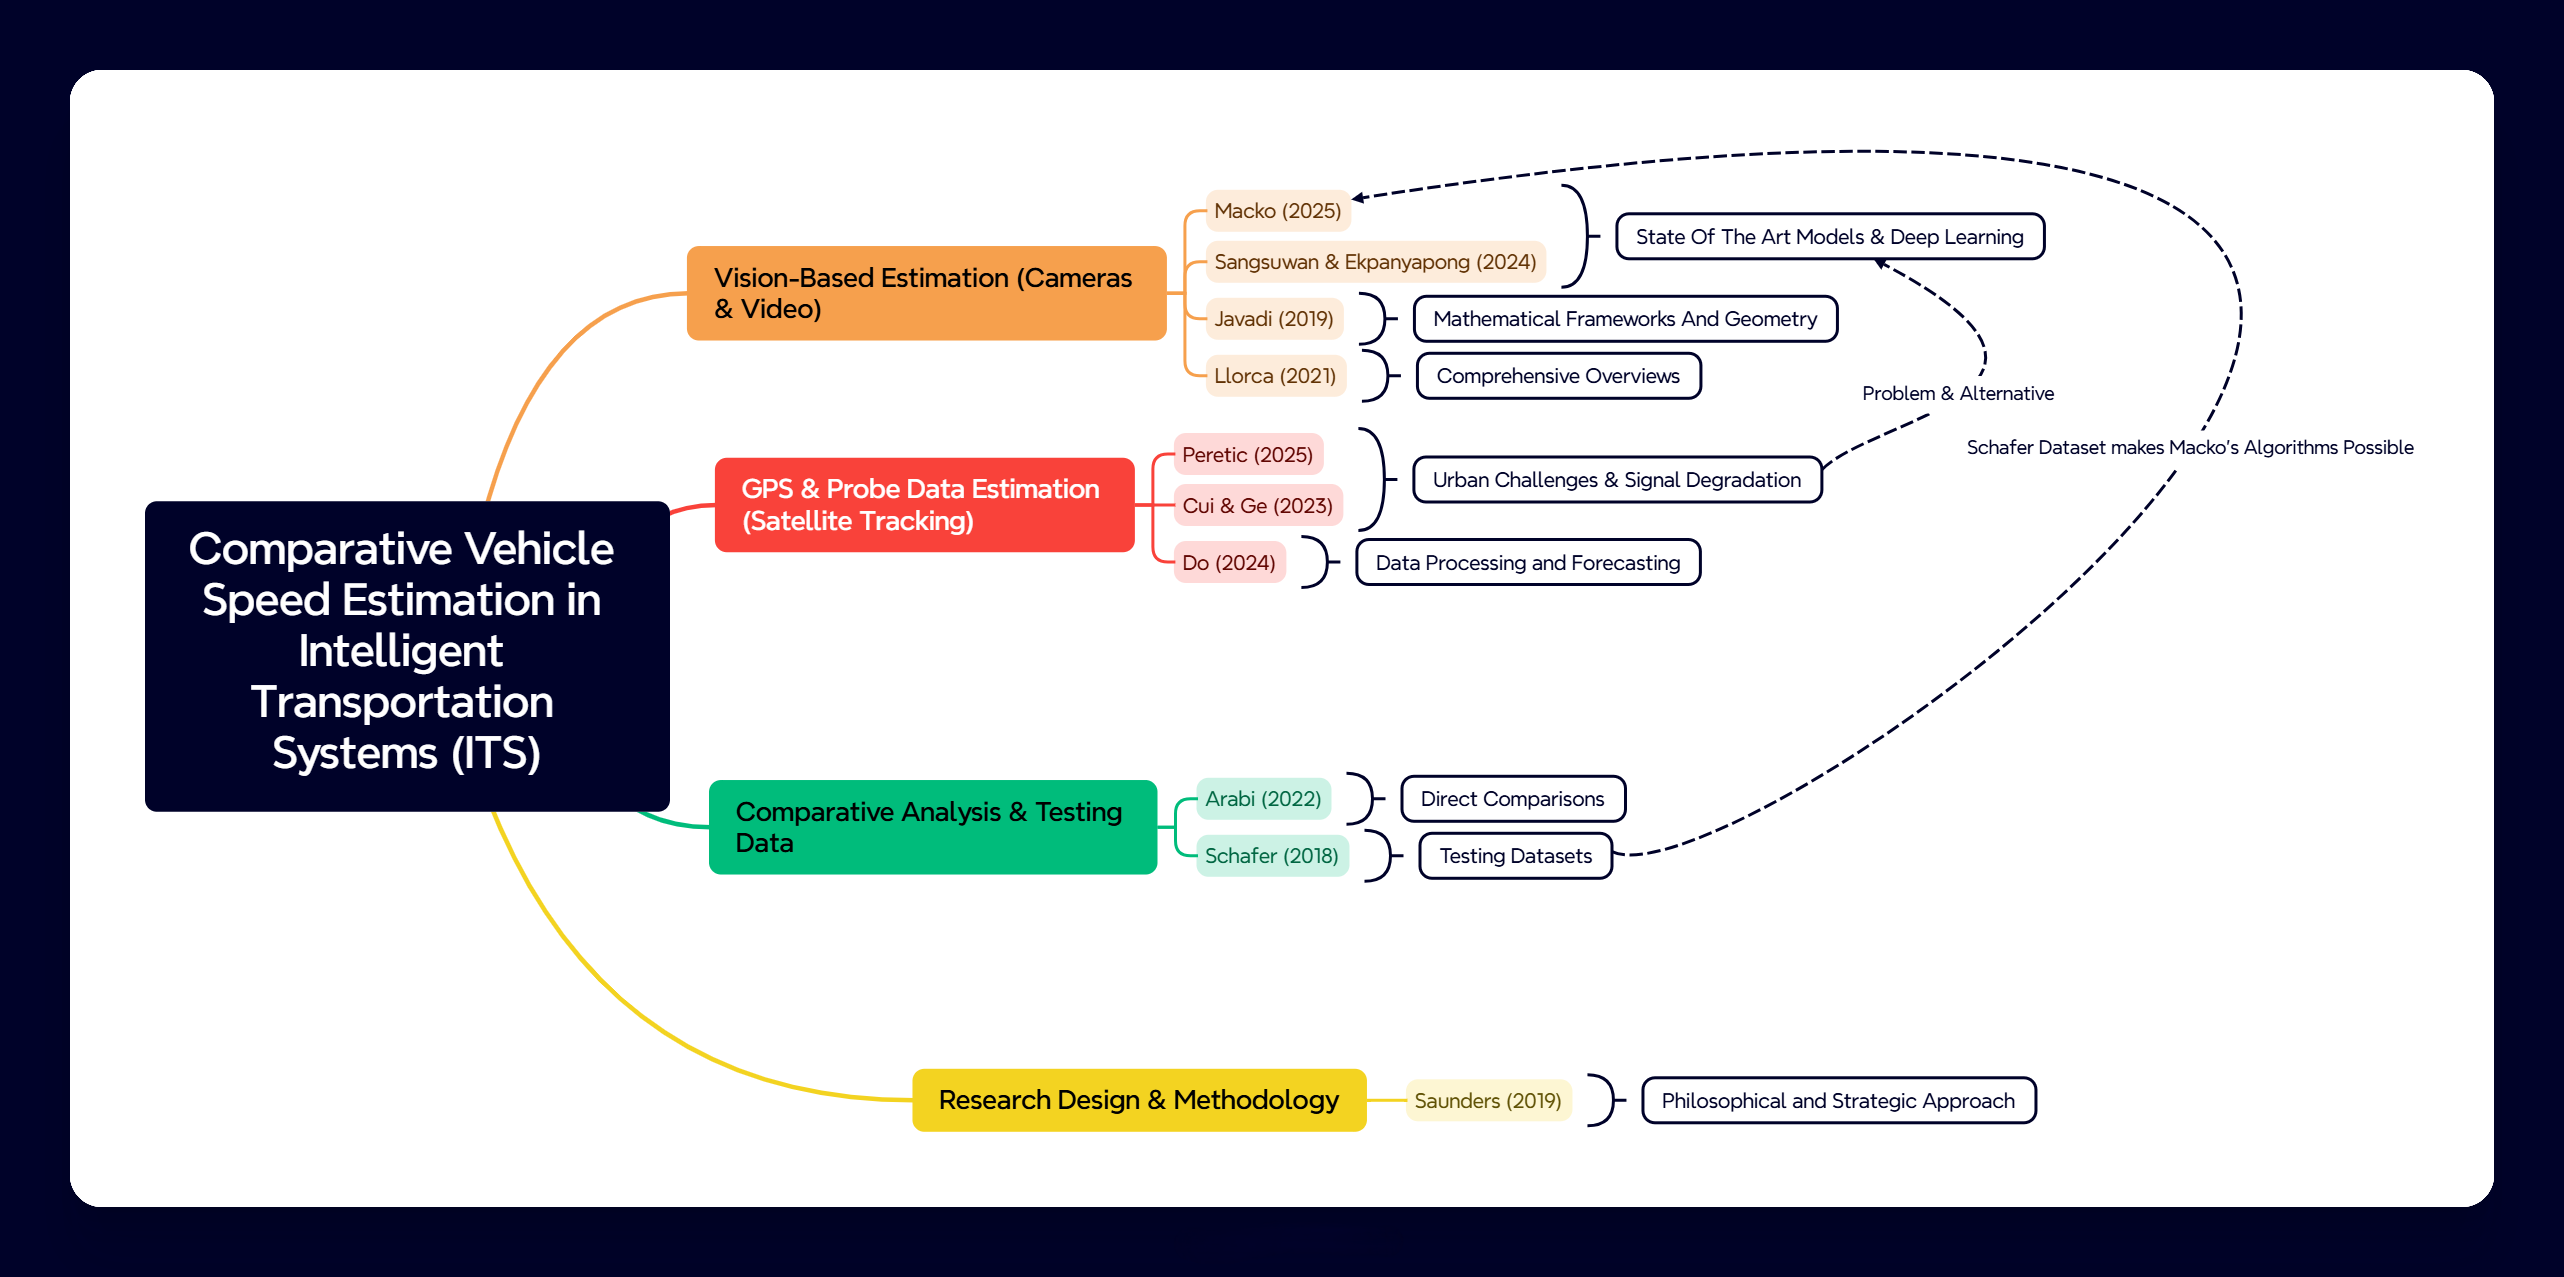
\includegraphics[width=\columnwidth]{includes/literaturemap.png}
    \caption{Literature Map}
    \label{fig:LiteratureMap}
\end{figure}
In the field of Intelligent Transportation Systems (ITS), the selected methodology fundamentally determines the accuracy of speed estimation. Looking into this research area, you can spot two main methods. Researchers focusing on vision-based speed estimation usually take an experimental, deductive approach based on positivism. Their methods generally entails the collection of primary data through edge-computing cameras, utilising geometric transformations (such as Inverse Perspective Mapping) or pixel-tracking algorithms to ascertain speed based on observable physical displacement.

Conversely, researchers looking at GPS probe data often go for a second, more numbers-driven way of analysing things. Their methodology utilises extensive datasets comprising historical, crowdsourced vehicle trajectories. Instead of conducting real-time physical experiments, their focus is predominantly on statistical modelling, noise mitigation, and using map-matching algorithms to fix those multi-path errors that pop up in city areas.

\subsection{Testing Strategies in the Chosen Context}
To implement these methods, a review of the literature identifies three principal testing strategies utilised by researchers to evaluate speed estimation frameworks.

The initial approach is what they call Controlled Closed-Circuit Testing, whereby researchers typically initiate testing within controlled, sterilised environments. They drive their specially equipped vehicles at set speeds around a closed track. This method effectively removes extraneous variables such as traffic occlusion or unpredictable civilian driving behaviour, thereby facilitating a concentrated focus on the mathematical principles underpinning the vision or GPS algorithms.

The second approach is known as `In-The-Wild' Highway Deployment. To check how well it scales, researchers put cameras on busy motorway overpasses. This testing method relies on obtaining a substantial sample size of uninstrumented civilian vehicles. The speed info from the vision system is then compared with big-picture GPS data from third-party companies to see how accurate it is in real-world conditions and how much delay there might be.

The third method involves Synthetic Simulation (Digital Twins). Researchers are progressively utilising advanced rendering engines to artificially produce accurate bounding boxes and tracking data in fake extreme weather scenarios that would be hard to mimic in real life. This methodology serves as an effective means of advancing the mathematical boundaries of speed estimation algorithms.

\subsection{Experimental Variables and Hypothesis Validation}
No matter what testing approach you use, researchers need to carefully control and tweak certain experimental variables to prove their ideas. When it comes to independent variables in vision-based studies, they often mess around with the camera angle (pitch and yaw), how far away the camera is from the target, and things like lighting and weather to see how solid the system is. Conversely, in studies involving GPS technology, the primary independent variable manipulated is the `polling rate', defined as the frequency at which the GPS receiver records a coordinate.

Accompanying these inputs, the universally measured dependent variable across all studies is the calculated velocity, expressed in kilometres per hour (km/h) or metres per second (m/s), along with the error margin, which they usually measure using Root Mean Square Error (RMSE) or Mean Absolute Percentage Error (MAPE).

Furthermore, to institute control variables and prove an alternative hypothesis, such as the proposal that a vision-based model shows greater accuracy than conventional GPS. This is usually done by arming test vehicles with super-calibrated Real-Time Kinematic (RTK) GPS or using LiDAR speed guns. Finally, by isolating these variables, researchers can definitively discover the specific parameters under which their speed estimation models remain valid.

\subsection{Distinguishing Between Academic and Non-Academic Material}
When we're looking at these variables and methods, it's important to clearly distinguish between well-tested academic research driven by the industry that isn't academically reviewed. Academic material sourced from peer-reviewed journals, these studies offer transparent methods, publicly accessible datasets (such as BrnoCompSpeed), and standard error metrics. They candidly acknowledge limitations, including camera calibration drift and GPS multipath errors.

Non-academic material, such as industry white papers and promotional reports from ITS hardware manufacturers, offer valuable insights into real-world adoption. However, they often lack methodological transparency. Frequently, they present ``best-case scenario'' accuracy figures without sufficiently detailing the experimental constraints, thereby rendering them unsuitable for establishing a scientific baseline.

\subsection{Recommended Peer-Reviewed Articles}
The following five peer-reviewed articles establish the methodological foundation for the comparison of vision and GPS techniques, each representing distinct layers of Saunders' Research Onion. 

\cite{macko2025efficient} operate firmly within a positivist paradigm, employing an experimental strategy through the employment of YOLO object detection in conjunction with vanishing point geometry. This study exemplifies contemporary standards for quantitative methodologies and procedures, avoiding reliance solely on fixed road-width assumptions.

Additionally \cite{arabi2022comparison} offer a highly pertinent comparative methodology in their work ``Comparison of the GPS and Camera Distance Estimation''. Their research demonstrates a deductive approach, establishing a rigorous framework for experimental validation by utilising RTK GPS as an infallible ground truth to test alternative hypotheses against monocular camera estimations.

Furthermore, \cite{fernandez2021vision} is integral to its archival research strategy, delineating the methodological evolution in data collection and analysis techniques, from fundamental background subtraction to sophisticated deep learning and optical flow methods.

To effectively contextualise the alternative approach in \cite{do2024enhanced}, this study focuses extensively on the specific techniques and procedures necessary for overseeing the inherent noise and low polling rates characteristic of continuous GPS trajectory data, relying heavily on large-scale cross-sectional data collection.

Lastly, \cite{rahimi2018vehicle} employs a strict monomethod quantitative approach, explicitly detailing the mathematical methodology involving virtual intrusion lines and frame-by-frame displacement. This represents a practical realisation of the innermost layers of the research onion, offering a methodology directly applicable to the development of bounding box prototype designs.

\subsection{Critical Literature Arguments and Knowledge Gaps}
A critical synthesis of the literature reveals distinct trade-offs between the two methodologies. Vision-based approaches are often praised for their strong localisation and perfect coverage, capturing every passing vehicle. However, the literature frequently disparages these systems for their fragility. Mathematical calibration is readily compromised by camera vibrations, and accuracy diminishes substantially during nighttime or adverse weather conditions.

Conversely, GPS probe data methods are esteemed for their continuous, network-wide coverage and resilience to visual environmental factors. Nonetheless, GPS studies frequently emphasise notable spatial inaccuracies within urban canyon environments, primarily due to signal multipath errors, and these methods are often characterised by low rates.

\subsubsection{Identifying The Knowledge Gap}
While there's plenty of research looking at vision systems in really controlled settings and GPS on open roads, there's still a big gap when it comes to comparing their performance all at once in busy, complicated city environments. Most studies investigate a single technology while presuming the other to be an infallible ground truth. There is a conspicuous absence of empirical research that rigorously evaluates a hybrid tracking methodology, such as integrating YOLO bounding boxes for primary detection with precise pixel displacement techniques, measured directly against consumer-grade GPS data within a real-world urban bottleneck scenario.
\input{includes/04-Methodology}
% \section{Results, Analysis and Discussion}

\subsection{Presentation of Results}
In accordance with the established experimental methodology, the vision-based prototype utilised Region of Interest (ROI) Dense Optical Flow (Farnebäck algorithm) and dynamic affine calibration, evaluated alongside consumer-grade GPS trajectory data. Both estimations were assessed against the 100Hz CAN-bus ground truth data obtained from the \textit{comma2k19} dataset \cite{schafer2018commute}. The evaluation was carried out over a continuous urban driving segment (\textit{segment\_30}), characterised by varying vehicle speeds, dynamic lighting conditions, and urban infrastructure.

To assess the accuracy and reliability of both systems, three standard statistical metrics were computed: Mean Absolute Error (MAE), Root Mean Square Error (RMSE), and Mean Bias Error (MBE). The MAE offers a linear measure of the average magnitude of error, the RMSE emphasises larger variances and extreme outliers, and the MBE indicates the propensity of the system to overestimate or underestimate the true velocity.

The comprehensive statistical results for the evaluated segment are shown in Table \ref{tab:error_metrics}.

\begin{table}[htbp]
\centering
\caption{Comparative Error Metrics: Vision vs. GPS Speed Estimation}
\label{tab:error_metrics}
\begin{tabular}{|l|c|c|c|}
\hline
\textbf{Estimation Method} & \textbf{MAE (km/h)} & \textbf{RMSE (km/h)} & \textbf{MBE (km/h)} \\ \hline
\textbf{GPS Probe Data} & 1.68 & 2.44 & -1.43 \\ \hline
\textbf{Vision (Optical Flow)} & 4.50 & 5.87 & +3.73 \\ \hline
\end{tabular}
\end{table}

To visually aid in the analysis of these findings, Figure \ref{fig:eval_plot} displays the instantaneous speed estimates of both the GPS and Vision systems in relation to the CAN-bus baseline over the course of the segment, accompanied by a rolling error subplot.

\begin{figure}[htbp]
    \centering
    % \columnwidth forces it to perfectly fit inside just one column
    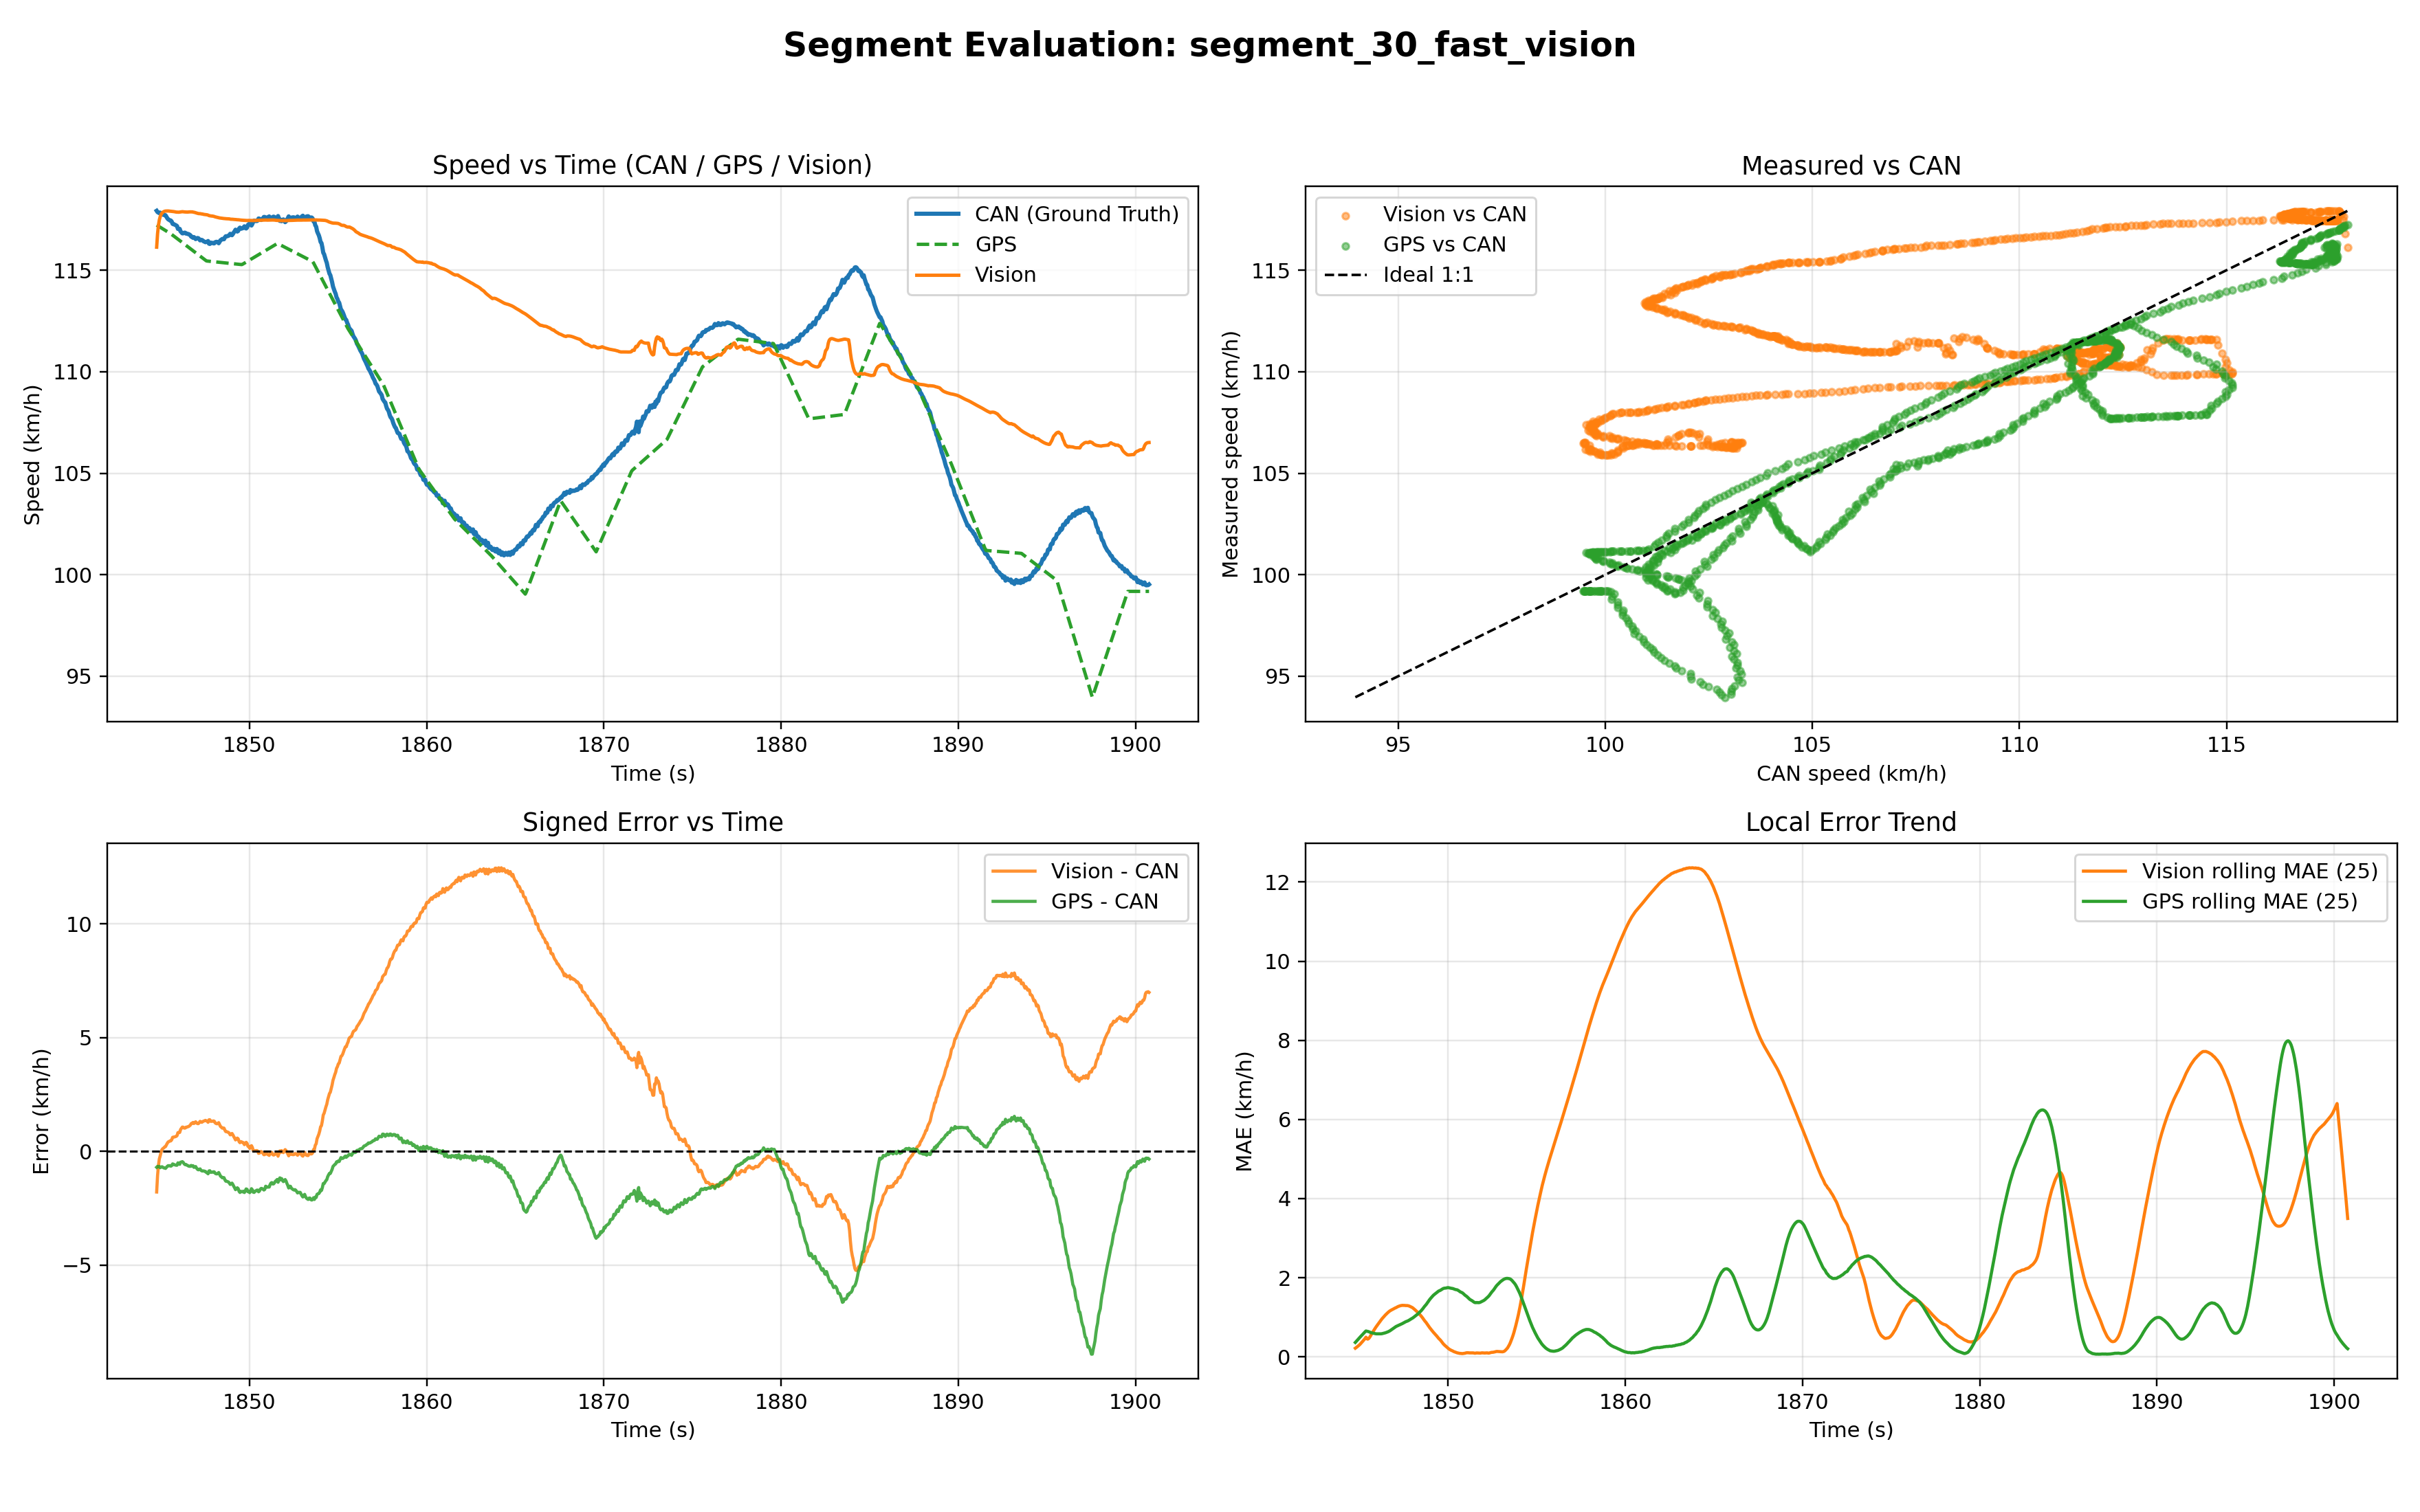
\includegraphics[width=\columnwidth]{includes/segment_30_fast_vision_evaluation.png} 
    \caption{Chronological comparison of GPS and Vision-based speed estimations against the CAN-bus ground truth, including instantaneous rolling error trends.}
    \label{fig:eval_plot}
\end{figure}
\subsection{Analysis and Interpretation of Results}
A detailed statistical analysis of the dataset indicates numerous significant behavioural patterns and technological correlations between the two speed estimation paradigms. The most notable and immediate finding from the data is that GPS trajectory estimations consistently exceeded the performance of the vision-based Dense Optical Flow pipeline across all measured metrics.

Observational analysis of the GPS data indicates a highly stable and notably consistent relationship with the CAN-bus ground truth. While consumer-grade GPS data has traditionally been associated with temporal latency, the interpolation and chronological frame alignment performed during the preprocessing phase effectively mitigated this issue. The GPS trace demonstrated a seamless correlation with the vehicle's true kinematics, resulting in an exceptionally low Mean Absolute Error (MAE) of 1.68 km/h. Additionally, the Root Mean Square Error (RMSE) score of 2.44 km/h suggests an absence of significant outliers; the GPS system did not experience substantial estimation failures during the segment, thereby demonstrating robust environmental stability. Interestingly, the GPS estimates exhibited a negative Mean Bias Error of -1.43 km/h. Cross-referencing the descriptive statistics reveals a mean GPS speed of 106.96 km/h, compared to the CAN-bus mean of 108.39 km/h. This minor systemic underestimation indicates a slight spatial lag during high-speed acceleration phases; however, its standard deviation (5.96 km/h) closely matched the vehicle's actual standard deviation (5.87 km/h), indicating that the GPS system accurately captured the full dynamic range of the drive.

Conversely, the vision-based pipeline exhibited considerable volatility and an incapacity to accurately track the vehicle's true dynamic range. The Farnebäck algorithm determines pixel intensity displacements on a frame-by-frame basis; however, the data indicate that this purely pixel-tracking approach is markedly unstable. The visual estimations produced a mean absolute error (MAE) of 4.50 km/h and a root mean square error (RMSE) of 5.87 km/h, rendering it nearly three times less precise than the GPS module.

A more detailed examination of the descriptive statistics reveals the precise nature of the failure within the vision system. The CAN-bus ground truth recorded a minimum speed of 99.47 km/h during a deceleration event, whereas the vision system’s minimum recorded speed was never less than 105.89 km/h. Additionally, the standard deviation of the visual output was only 3.72 km/h, in contrast to the actual standard deviation of 5.87 km/h. This suggests a significant `flattening' effect. The optical flow algorithm compressed the speed range and failed entirely to detect deceleration. When the vehicle reduced its speed, the forward pixel displacement should have decreased proportionally; however, environmental visual noise, such as the relative motion of passing vehicles, lane markings blurring at high speeds, and shifts in lighting, maintained the average pixel magnitude at artificially elevated levels. This fundamental deficiency in the algorithm’s lack of semantic understanding resulted in a substantial systemic overestimation of speed, evidenced by a positive Mean Bias Error (MBE) of +3.73 km/h.

\subsection{Comparison, Contrast and Comment on Findings (Critique)}
When comparing the two methodologies, it is apparent that, although vision-based systems exhibit theoretical advantages in real-time kinematic responsiveness, their practical deployment employing purely pixel-tracking mathematics is exceedingly fragile. The GPS data demonstrated complete immunity to the visual environmental factors that compromised the optical flow system.

A critique of the methodology highlights strong experimental controls; however, it also identifies notable technological limitations pertaining to the vision prototype.

\begin{itemize}
    \item \textbf{Validity:} In accordance with the methodological frameworks outlined by Saunders et al. \cite{saunders2019research}, the internal and construct validity of these findings is of an exceptionally high standard. Utilising the \textit{comma2k19} dataset \cite{schafer2018commute}, the temporal synchronisation between the camera, GPS, and CAN-bus was assured. Consequently, the results accurately reflect the true algorithmic precision of the sensors, rather than being influenced by arbitrary synchronisation errors or extraneous human factors.
    \item \textbf{Reliability:} The computational reliability of the Python pipeline is guaranteed; the deterministic nature of the mathematical tracking ensures that executing the code repeatedly produces identical pixel displacements. However, the environmental reliability of the vision system is highly limited. As it relies solely on pixel gradients, minor changes such as a shadow passing across the dashboard or a glare on the windscreen can artificially distort the velocity matrix.
    \item \textbf{Generalisability (Transferability):} This continues to represent a significant limitation of the findings. The experiment was conducted on a specific dataset primarily recorded in well-lit Californian highway environments \cite{schafer2018commute}. Given that the optical flow pipeline systematically failed to detect deceleration under ideal, clear weather conditions, its applicability to adverse weather conditions is effectively nil. Heavy precipitation, fog, or night-time driving fundamentally alter pixel intensities, which would cause the performance of the Farnebäck algorithm to deteriorate exponentially within a broader real-world context.
\end{itemize}

\subsection{Discussion in Relation to Original Hypothesis and Existing Literature}
The original alternative hypothesis of this research proposed that the vision-based method would achieve a smaller margin of error compared to GPS during normal driving, owing to the inherent latency, multipath errors, and noise associated with commercial GPS receivers. However, based on the definitive comparative metrics (GPS Mean Absolute Error 1.68 km/h versus Vision Mean Absolute Error 4.50 km/h), the alternative hypothesis is wholly rejected, thereby overturning the null hypothesis in the opposite direction: GPS probe data is markedly superior to Dense Optical Flow for the estimation of vehicle speed.

These findings present a compelling intersection with the environmental constraints extensively discussed in the existing literature. Foundational studies by Cui and Ge \cite{cui2003autonomous} and recent statistical analyses by Li et al. \cite{li2025statistical} document the severe degradation of GNSS signals within urban canyons attributable to multipath signal reflection. While the literature correctly identifies the vulnerability of GPS in areas of significant occlusion, empirical data from this study demonstrates that, beyond the confines of severe urban canyons, standard GPS probe data remains notably accurate and dependable. The marginal negative bias (MBE: -1.43 km/h) observed aligns with the latency concerns highlighted by Cui and Ge \cite{cui2003autonomous}, yet it was not sufficiently substantial to undermine the overall accuracy of the estimations.

Furthermore, the failure of the visual pipeline provides significant context for the methodological evolution outlined by Fernandez Llorca et al. \cite{fernandez2021vision} and the virtual intrusion line mathematics proposed by Rahimi \cite{rahimi2018vehicle}. While Rahimi \cite{rahimi2018vehicle} demonstrated that frame-by-frame displacement constitutes a mathematically sound concept in highly controlled, stationary camera configurations, this experiment illustrates that applying dense optical flow to a moving ego-vehicle introduces an insurmountable level of dynamic noise. In the absence of the capacity to distinguish between the road surface approaching the camera and another vehicle moving laterally across the frame, pure optical flow tends to overestimate physical velocity. This observation strongly corroborates the findings of Arabi et al. \cite{arabi2022comparison}, who underscored the critical importance of reliable ground truth data, in uncovering the underlying fragilities inherent to monocular camera estimations.

\subsection{Evaluation of the Approach and Future Implementations}
Assessing this overarching research approach in comparison with the methodologies employed by other contemporary researchers illuminates evident pathways for future applications. The choice to utilise Dense Optical Flow emphasised the limitations inherent in classical computer vision techniques.

As demonstrated by Macko et al. \cite{macko2025efficient}, the industry is rapidly shifting towards deep learning paradigms, notably utilising YOLO object detection frameworks. Although the optical flow approach employed in this study is computationally lightweight and does not necessitate extensive datasets for neural network training, it fundamentally lacks semantic comprehension. A YOLO-based system, as advocated by Macko et al. \cite{macko2025efficient}, delineates the discrete, physical boundaries of specific vehicles. By isolating a bounding box, a YOLO model exhibits considerable resilience to shadows, oncoming traffic, and peripheral visual noise, which previously resulted in significant error spikes and a "flattened" deceleration curve within this study's optical flow data.

Furthermore, researchers specialising in GPS probe data, such as Do et al. \cite{do2024enhanced}, have demonstrated that raw trajectory data can be significantly optimised through the application of Deep Neural Networks to forecast and smooth multipath errors. This indicates that the raw, uninstrumented GPS data employed in this experiment could be further refined towards near-perfect accuracy via algorithmic noise reduction. P. P. et al. \cite{pp2024video} also endorse the view that raw speed measurement metrics must be continuously enhanced through advanced contextual filtering.

Consequently, an enhanced approach for future applications of this research should eschew the mutually exclusive comparison of these technologies in favour of Sensor Fusion. As evidenced by the data, GPS offers absolute and relatively stable physical positioning but is affected by marginal latency and slight underestimations during dynamic movements \cite{cui2003autonomous, li2025statistical}. Conversely, camera-based data exhibits instantaneous kinematic responsiveness; however, it is highly susceptible to visual fragility and tends to overestimate positive biases.

Future research should incorporate a Kalman Filter architecture, a sophisticated statistical algorithm designed to seamlessly integrate multiple noisy data streams. By leveraging GPS data to establish the steady-state speed and employing a YOLO-masked optical flow pipeline to rectify transient instantaneous errors, a hybrid prototype could attain accuracy within sub-1 km/h margins. This data fusion approach would mitigate the individual limitations associated with satellite-based and vision-based methods identified in this study, thereby representing a crucial advancement in the evolution of perception systems for autonomous vehicles.
% \section{Conclusion}

\subsection{Main Conclusion and Hypothesis Evaluation}
This research critically evaluated the relative accuracy of vision-based and GPS-based speed estimation algorithms for autonomous vehicles. The principal inquiry examined the performance of a vision-based model, employing Region of Interest (ROI) Dense Optical Flow and dynamic affine calibration, in comparison to conventional GPS probe data against a CAN-bus ground truth.

The principal conclusion is unequivocal: consumer-grade GPS trajectory data markedly surpasses the proposed pixel-tracking vision methodology in terms of both accuracy and stability. The GPS-based pipeline attained a Mean Absolute Error (MAE) of 1.68 km/h, whereas the vision-based system yielded an MAE of 4.50 km/h, demonstrating that the optical flow approach is nearly three times less precise.

These findings definitively refute the original research hypothesis, which proposed that the vision-based method would result in a smaller error margin owing to satellite latency. The data indicate that, although GPS exhibits a slight negative bias of -1.43 km/h, its overall ability to accurately ascertain a vehicle’s kinematics in typical urban environments is significantly superior to that of Dense Optical Flow.

\subsection{Shortcomings in the Methodology}
While the setup benefited from the highly synchronised ground truth provided by the \textit{comma2k19} dataset \cite{schafer2018commute}, a thorough evaluation reveals several important methodological limitations.

\subsubsection{Algorithmic Fragility}
Relying on the Farnebäck algorithm meant tracking raw visual shifts rather than physical objects. The methodology failed to account for environmental visual noise, such as bridge shadows and oncoming traffic. This lack of semantic understanding caused the algorithm to fail at detecting deceleration, resulting in a systemic overestimation of speed.

\subsubsection{Limited Generalisability}
The dataset exhibited well-illuminated, clear Californian weather conditions. As the optical flow methodology deteriorates during slight variations in lighting even under optimal circumstances, its efficacy in adverse weather conditions or during nocturnal driving would be substantially compromised.

\subsubsection{Camera Calibration Assumptions}
The dynamic affine calibration mathematically presumes a stable camera pitch. In practice, intense braking induces suspension dive, which alters the pitch and compromises the integrity of the optical flow vectors. The methodology did not incorporate pitch-compensation algorithms to address this physical variable.

\subsection{Suggestions for Further Research}
To further the development of Intelligent Transportation Systems (ITS), several promising avenues for additional research present themselves:

\subsubsection{Transition to Deep Learning (YOLO)}
Future vision-based research should incorporate deep learning frameworks such as YOLO (You Only Look Once) for object detection. By precisely monitoring the physical boundaries of a vehicle, the system attains a semantic understanding, thereby enabling it to disregard peripheral visual noise and shadows that previously compromised the effectiveness of optical flow techniques.

\subsubsection{Sensor Fusion via Kalman Filtering}
Research should shift from assessing GPS and vision as mutually exclusive solutions towards their active integration. GPS offers reliable positioning but is subject to slight latency, whereas camera data provides immediate responsiveness but remains environmentally sensitive. The utilisation of a Kalman Filter to combine these data streams could theoretically attain error margins below 1 km/h.

\subsubsection{Algorithmic Noise Mitigation for GPS}
Considering that raw GPS data demonstrated exceptional performance, future research efforts should focus on employing Deep Neural Networks (DNNs) with standard satellite trajectories in order to predict and mitigate multipath signal reflections, thereby advancing consumer-grade receivers towards near-Real Time Kinematic (RTK) accuracy.

\appendices
% \input{includes/07-Supporting}
% \section*{Acknowledgement}

This article was developed with the assistance of artificial intelligence tools (such as ChatGPT), which were employed solely for tasks including language editing, textual revision, and initial information structuring. The application of these tools was strictly instrumental; they did not substitute the authors' critical analysis, data interpretation, methodological choices, or scientific responsibility. The authors retain full accountability for the authorship and integrity of the content provided herein.

You can dedicate this section for special assistance that you were given by a 3rd party. Not your mentor, relatives or questionnaire participants.

\bibliographystyle{IEEEtran}
\bibliography{sources}

\end{document}


